\documentclass[a4paper,
fontsize=11pt,
%headings=small,
oneside,
numbers=noperiodatend,
parskip=half-,
bibliography=totoc,
final
]{scrartcl}

\usepackage[babel]{csquotes}
\usepackage{synttree}
\usepackage{graphicx}
\setkeys{Gin}{width=.4\textwidth} %default pics size

\graphicspath{{./plots/}}
\usepackage[ngerman]{babel}
\usepackage[T1]{fontenc}
%\usepackage{amsmath}
\usepackage[utf8x]{inputenc}
\usepackage [hyphens]{url}
\usepackage{booktabs} 
\usepackage[left=2.4cm,right=2.4cm,top=2.3cm,bottom=2cm,includeheadfoot]{geometry}
\usepackage[labelformat=empty]{caption} % option 'labelformat=empty]' to surpress adding "Abbildung 1:" or "Figure 1" before each caption / use parameter '\captionsetup{labelformat=empty}' instead to change this for just one caption
\usepackage{eurosym}
\usepackage{multirow}
\usepackage[ngerman]{varioref}
\setcapindent{1em}
\renewcommand{\labelitemi}{--}
\usepackage{paralist}
\usepackage{pdfpages}
\usepackage{lscape}
\usepackage{float}
\usepackage{acronym}
\usepackage{eurosym}
\usepackage{longtable,lscape}
\usepackage{mathpazo}
\usepackage[normalem]{ulem} %emphasize weiterhin kursiv
\usepackage[flushmargin,ragged]{footmisc} % left align footnote
\usepackage{ccicons} 
\setcapindent{0pt} % no indentation in captions
\usepackage{xurl} % Breaks URLs

%%%% fancy LIBREAS URL color 
\usepackage{xcolor}
\definecolor{libreas}{RGB}{112,0,0}

\usepackage{listings}

\urlstyle{same}  % don't use monospace font for urls

\usepackage[fleqn]{amsmath}

%adjust fontsize for part

\usepackage{sectsty}
\partfont{\large}

%Das BibTeX-Zeichen mit \BibTeX setzen:
\def\symbol#1{\char #1\relax}
\def\bsl{{\tt\symbol{'134}}}
\def\BibTeX{{\rm B\kern-.05em{\sc i\kern-.025em b}\kern-.08em
    T\kern-.1667em\lower.7ex\hbox{E}\kern-.125emX}}

\usepackage{fancyhdr}
\fancyhf{}
\pagestyle{fancyplain}
\fancyhead[R]{\thepage}

% make sure bookmarks are created eventough sections are not numbered!
% uncommend if sections are numbered (bookmarks created by default)
\makeatletter
\renewcommand\@seccntformat[1]{}
\makeatother

% typo setup
\clubpenalty = 10000
\widowpenalty = 10000
\displaywidowpenalty = 10000

\usepackage{accessibility}
\usepackage[colorlinks, linkcolor=black,citecolor=black, urlcolor=libreas,
breaklinks= true,bookmarks=true,bookmarksopen=true]{hyperref}
\usepackage{hyperxmp}
\usepackage{breakurl}

%meta
%meta

\fancyhead[L]{Redaktion LIBREAS\\ %author
LIBREAS. Library Ideas, 48 (2026). % journal, issue, volume.
\href{https://doi.org/10.18452/37897}{\color{black}https://doi.org/10.18452/37897}
{}} % doi 
\fancyhead[R]{\thepage} %page number
\fancyfoot[L] {\ccLogo \ccAttribution\ \href{https://creativecommons.org/licenses/by/4.0/}{\color{black}Creative Commons BY 4.0}}  %licence
\fancyfoot[R] {ISSN: 1860-7950}

\title{\LARGE{Auf einen Espresso mit Dirk Wissen}}% title
\author{Dirk Wissen, Linda Freyberg} % author

\setcounter{page}{1}

\hypersetup{%
      pdftitle={Auf einen Espresso mit Dirk Wissen},
      pdfauthor={Dirk Wissen, Linda Freyberg},
      pdfsubject={LIBREAS. Library Ideas, 48 (2026)},
      pdfkeywords={Interviews, BuB, Bibliotheken, Atmosphäre},
      pdflicenseurl={https://creativecommons.org/licenses/by/4.0/},
      pdfcopyright={CC BY 4.0 International},
      pdfcontacturl={http://libreas.eu},
      pdfurl={https://doi.org/10.18452/37897},
      pdfdoi={10.18452/37897},
      pdflang={de},
      pdfmetalang={de}
     }



\date{}
\begin{document}

\maketitle
\thispagestyle{fancyplain} 

%abstracts
\begin{abstract}
\noindent
Interview geführt von Linda Freyberg an einem lauen Sommerabend am 3.
Juni 2026 in Berlin-Friedrichshain. In BuB erschien seit 2015 monatlich
die Interviewreihe \enquote{Wissen fragt \ldots{} auf einen Espresso mit
\ldots{}}, in dessen Rahmen er 102 Interviews zum Thema \enquote{Atmosphäre
von Bibliotheken} führte.
\end{abstract}

%body
\textbf{Vorbemerkung}

Dr.~Dirk Wissen ist promovierter Bibliotheks- und
Literaturwissenschaftler sowie leidenschaftlicher Bibliothekar. Seine
Dissertation hat den Titel \enquote{Zukunft der Bibliographie --
Bibliographie der Zukunft}. Wissen ist seit 30 Jahren Mitglied des BIB --
Berufsverband Information Bibliothek e.\,V., bei dem er zehn Jahre, von
2015 bis 2026, Mitglied im BIB-Bundesvorstand und Herausgeber der Fach-
und Verbandszeitschrift \enquote{BuB -- Forum Bibliothek und
Information} war. In BuB erschien seit 2015 monatlich die Interviewreihe
\enquote{Wissen fragt \ldots{} auf einen Espresso mit \ldots{}}, in
dessen Rahmen er 102 Interviews zum Thema \enquote{Atmosphäre von
Bibliotheken} führte.

\begin{figure}[h!]
\centering
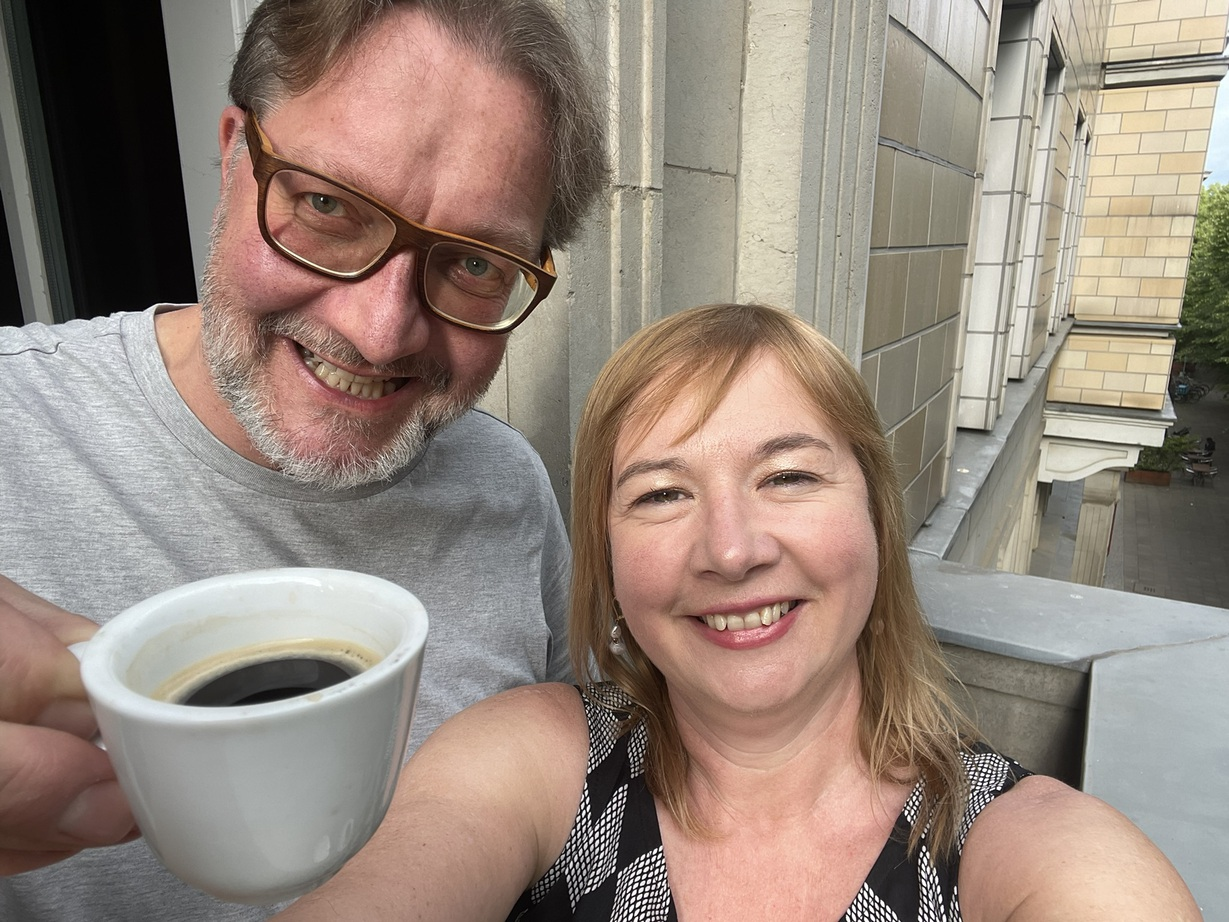
\includegraphics[width=0.8\textwidth,keepaspectratio]{img/foto-dirk-linda.jpeg}
\caption{Abbildung 1: Auf einen Espresso mit Dirk Wissen}
\alt{Ein Selfie von Dirk Wissen und Linda Freyberg. Beide lächeln in die Kamera und Dirk Wissen hält eine Tasse mit Espesso vor die Linse.}
\end{figure}

\emph{Linda Freyberg (LF): Zunächst zu den Anfängen: Seit 2009 hattest
du eine Gesprächsreihe im Rahmen von Lesungen und Neuerscheinungen.}

Dirk Wissen (DW): Ja, es gab regelmäßig und jahrelang jeden Monat in
Frankfurt (Oder) ein Format, das noch nicht \enquote{Wissen fragt
\ldots{}} hieß, sondern \enquote{Wissen trifft \ldots{}}, wo auch
namhafte Schriftstellerinnen und Schriftsteller wie Erich Loest und Juli
Zeh nach Frankfurt (Oder) kamen. Und Literaturveranstaltungen moderierte
ich bereits eine Zeit lang vorher in Münster und Würzburg.

Auch Martin Walser hatte seinen Weg vom Bodensee extra nach Frankfurt
(Oder) gemacht, was zu sehr schönen, mir in Erinnerung bleibenden
Momenten kam. Er und andere mussten ja dann auch aus Frankfurt (Oder)
wieder zurückkommen und reise mal gegen 22 Uhr aus Frankfurt (Oder) zum
Bodensee zurück. Er brauchte natürlich ein Hotel und so gab es eine
gemeinsame Zugfahrt zurück bis nach Berlin.

So war es auch mit dem heutigen Bestseller-Autor Benedict Wells. Wir
saßen gemeinsam im Zug und sprachen über Legasthenie und
Analphabetismus, also über ganz andere Themen als in seinem Debütroman
beziehungsweise worum es damals auf der Bühne ging. Und dann habe ich
gesagt, dass ich auch irgendwie etwas Autistisches habe und dass ich
beim Schreiben selber sehr viele Fehler mache, aber komischerweise
Fehler in Büchern sofort sehe. Das wollte er erst nicht glauben und gab
mir sein Buch. Ich blätterte es durch und sagte, hier ist ein
Tippfehler. Also wirklich in Sekunden und dann hatten wir so ein Thema
und er schenkte mir sein Buch und verriet mir, bei welchen Textstellen
er auch weiß, dass da Fehler enthalten sind. Das Buch wurde mit
zahlreichen lustigen Korrekturanmerkungen versehen und steht hier mit
Widmung in meinem Bücherregal.

\emph{LF: Und wie ist das dann 2015 von dieser Gesprächsreihe zum
Interviewformat in der BuB \enquote{Wissen fragt \ldots{}} gekommen?}

DW: Da war ich noch gar nicht Herausgeber dieser Zeitschrift. Ich fand
das BuB seit meinen Studienanfängen einfach toll, aber es hat ja auch
Wechsel gegeben vom Format und von den Inhalten. Und irgendwann dachte
ich mir, dass es ja immer diese Best Practice Beispiele und Interviews
von dem und dem Bibliotheksdirektor oder -direktorin gab. Da habe ich
der Redaktion eine E-Mail geschrieben, was sie davon halten würde, wenn
man mal ab und zu Interviews führt mit einem Architekten, der gerade
wieder eine Bibliothek baut, aber vielleicht diese nie nutzt, um Bücher
auszuleihen oder einem Schriftsteller wie Martin Walser, von dem ein
ganzes Bücherregal in den Öffentlichen Bibliotheken steht, dem das aber
möglicherweise gar nicht bewusst ist, wie so eine \enquote{Walser-Wand}
aussieht. Und dann kam zurück: Ja, mach das mal, fünfmal. Die ersten
fünf Interviews waren kompakt und schnell fertig, auch weil ich so eine
Sicherheit wollte, dass das hintereinander weg funktioniert. Und dann
gabs die Antwort, dass ich mal weiter machen solle, da waren diese noch
gar nicht publiziert. Und glücklicherweise gab es später nicht einen
kritischen Leserbrief, aber sehr viel positives Feedback im Laufe der
Jahre.

\emph{LF: Also basiert die Reihe auf deiner Initiative und deinem
Konzept?}

DW: Ja, unter anderem die Idee, dass die letzte These, Fragestellung
oder Problematik eines Interviewpartners, die genannt wird, an den
nächsten weitergereicht wird. Und dass es immer einen Espresso gibt.
Auch dass es ein Kurzinterview sein sollte und möglichst nie jemand aus der
Politik oder eine Bibliothekskollegin oder -kollege interviewt werden sollte, aber es immer
einen Bibliotheksbezug geben sollte, wie eben beim Architekten Max
Dudler mit seinen Bibliotheksbauten. Wichtig war mir dabei immer, dass die Fotos der Bibliotheken von
mir stammten, so dass ich nach Stockholm bin, um in der Stadtbibliothek
die Rotunde oder nach Oslo, um die Jugendbibliothek Tøyen zu
fotografieren -- welche als Erwachsener gar nicht betreten werden darf,
wozu Aat Vos extra eine Mail an die Bibliotheksleitung für mich schrieb.

\emph{LF: Und so entstanden dann 102 sehr vielseitige Interviews, vor
allem mit Schriftsteller*innen, was ja nicht so überraschend ist, da du
ja in der Literaturwissenschaft promoviert hast. Es war sogar eine
Literaturnobelpreisträgerin dabei: Swetlana Alexandrowna Alexijewitsch.
Wie war das denn mit ihr?}

DW: Das war das 13te publizierte Interview in der Reihe. Nachdem sie
gerade ihren Literaturnobelpreis erhalten hatte, saß ich bei ihr in
einer Veranstaltung und stellte eine Publikumsfrage. Und hinterher sind
dann sehr viele Leute für ein Autogramm angestanden, um sich ihr Buch
signieren zu lassen. Und ich stand dazwischen. Bei mir schaut sie auf
einmal hoch und sagte: \enquote{Sie waren doch der aus dem Publikum mit
dieser interessanten Frage zur Freiheit. Mit ihnen würde ich mich ja
gern länger unterhalten.} -- was die Übersetzerin übersetzte, da ich
kein Wort Russisch spreche. Meinerseits sagte ich, dass dies gerne
möglich sei und auch als Interview publiziert werden könne, da es gerade
diese Anfrage von BuB gab, die bis dahin noch unveröffentlichte
Interviewreihe weiterzuführen. Das führte dann dazu, dass sie für ein
Gespräch in Berlin Wochen später zusagte. An dem Tag führte sie
dann mehrere Interviews -- vor mir war die taz, danach die FAZ, und das
Schweizer Fernsehen und so weiter. Sie hatte also den ganzen Tag
Interviews geführt, ähnlich wie Hugh Grant in Notting Hill, als er für
das Gespräch mit Julia Roberts sagt, er käme von \enquote{Horse \&
Hound}. Und hinterher, da bin ich heute noch gerührt davon, bekam ich
eine E-Mail, dass sie sich am meisten an diesem Tag über mein Interview
gefreut hätte. Vielleicht, weil ich überhaupt nicht über ihre Bücher mit
ihr gesprochen hatte, obwohl sie aus meiner Frage bei der Veranstaltung
wusste, dass ich die gelesen hatte. Aus irgendeinem Grund haben wir uns
nur über Bibliotheken unterhalten und das fand sie toll.

Und genau zu dieser Zeit begann es auch mit den Selfies, die die
Interviewpartner mit mir machten -- so habe ich auch einfach ein Selfie
gemacht. Zeitgleich gab es dann in einer sehr bekannten Musikzeitschrift
Fake-Interviews. Da dachte ich mir, das glaubt dir ja niemand, dass du
innerhalb einer Woche Max Dudler, den Architekten und Alexijewitsch, die
Nobelpreisträgerin getroffen hast und habe dann die Selfies mit der
Espressotasse, quasi als Beweis, an die BuB-Redaktion mit den Texten
mitgeschickt. Dass die das dann zum Abdrucken verwendeten, überraschte
mich -- und dann wurde es wie zu einem Markenzeichen.

\emph{LF: Aber von den ersten Interviews gab es noch keine Selfies?}

Doch, seit dem zweiten. Ich hatte quasi von Anfang an mit jedem ein
Selfie als Erinnerung gemacht, weil sie selber auch mit mir eines
gemacht hatten. Das war 2015 doch wie ein Trend. Und das Interview mit
Frau Alexijewitsch war das sechste Gespräch, wurde aber erst viele
Monate später zur Buchmessenausgabe von BuB gedruckt. Und mit dem ersten
Interviewpartner habe ich mich einfach nochmal getroffen. Wir waren
befreundet, das war der Philosoph Antoine Verbij.

Das ist leider auch eine traurige Geschichte: Ich habe mit ihm privat
ein Gespräch geführt, und zwar einfach, weil wir uns kennengelernt
hatten, als er über Döblins \enquote{Berlin Alexanderplatz} etwas
schreiben wollte. Ich führte ihn zu den Biberkopf-Orten und so lernten
wir uns privat kennen. Er ist auch Journalist und Publizist und einmal
sagte er dann zu mir \enquote{das Gespräch, welches wir gerade führen,
mit deinen Fragen zu Bibliotheken, das solltest du publizieren}. Also
hat er mich im Grunde auf diese Idee gebracht. Wir haben dann noch
gemeinsam verschiedene Veranstaltungen organisiert, unter anderem eine
mit der holländischen Botschaft und ich habe ihm geholfen für seinen
Artikel, der anlässlich des erstmaligen Erscheinens einer
niederländischsprachigen Gesamtausgabe von \enquote{Berlin
Alexanderplatz} in einer holländischen Zeitung erschien. Wie gesagt, da
bin ich mit ihm durch ganz Berlin spaziert, habe ihm reale Orte, die im
Roman benannt werden, gezeigt, wie die \enquote{Neue Welt} in dessen
Zusammenhang Chaplin genannt wird -- und wir haben uns einfach von
Beginn an sehr gut verstanden. Doch das Traurige ist, er hat noch den
Interviewtext freigegeben und verstarb eine Woche bevor das Heft
publiziert wurde. Das hat emotional mit mir etwas gemacht und ich
dachte, ich muss diese Idee weiterführen und dann ging das ja auch
101-mal weiter.

\emph{LF: Und wie lief dann im Folgenden die Akquise oder wie kamst du
auf die Personen? Bei den Schriftsteller*innen ist das ja relativ
naheliegend, weil du ja Interesse an Literatur hast und auf Lesungen
gehst, aber es waren ja auch ganz viele andere Berufsgruppen dabei:
Architekt*innen, eine Übersetzerin, ein Programmierer, Künstler*innen,
viele Musiker*innen, Wissenschaftler*innen, und sogar mal ein Roboter
und eine KI.}

\emph{Gerade bei fachfremden Personen war es wahrscheinlich immer recht
unterschiedlich, wie du mit denen in Kontakt gekommen bist. Kannst du
über diesen Prozess etwas erzählen?}

DW: Also ich habe meistens versucht den persönlichen Kontakt
herzustellen, wenn es eine Veranstaltung gab. Das ist ja in Berlin im
Grunde jeden Tag möglich. Was ich aber auch gemacht habe, ist, mich ganz
offiziell an das Management zu wenden mit Informationen zu der
Fachzeitschrift und der Interviewreihe. Das führte dann manchmal dazu,
dass im Vorfeld vom Management mehr Fragen aufkamen, als ich für das
eigentliche Interview vorgesehen hatte. Und deswegen sind natürlich auch
einige Interviews gar nicht zustande gekommen. So wusste ich
beispielsweise bei der Sängerin Balbina, dass ich vorab nichts von der
Idee schreiben werde, zeitgleich ein dadaistisches Interview mit
\enquote{Anna Blume} führen zu wollen. Das habe ich dann die Künstlerin
einfach beim Interview gefragt, ob sie sich das vorstellen könne, wie es
dann ja auch publiziert wurde.

\emph{LF: Möchtest du verraten, an wen es am Schwierigsten war,
ranzukommen?}

DW: Ja, das war Karl-Ove Knausgård, dessen Bücher ich alle gelesen habe,
und mir die Mühe gemacht hatte, jede Bibliothek, die er in seinen
Büchern nennt, in einer Liste aufzuschreiben, damals noch händisch ganz
ohne KI. Es sollte um das Thema \enquote{Volltextrecherche} gehen. Und
diese Liste habe ich ihm bei einer Lesung gegeben und zwei Jahre später,
bei einer weiteren Lesung von ihm nochmal nachgefragt und so weiter --
es gibt mehrere Selfies mit ihm, aber kein Interview. Wir haben auch
miteinander gesprochen, aber das eigentliche Interview fand dann nicht
statt und das war natürlich mit einigen Personen so.

Aber das Positive ist, mit Vielen hat es sehr schnell funktioniert. In
dem Moment, wo ich jemanden angefragt habe, war ich immer am selben Tag
der Anfrage bereit, weil es sein konnte, dass es einen Anruf gab oder
nach einer Veranstaltung ich sofort für das Gespräch irgendwo mit hinkommen
sollte.

Es gab aber auch Interviews, für die ich lange im Voraus eine Anfrage
gestellt hatte. Volker Kutscher, den kennt man ja von der Verfilmung
seiner Romane durch \enquote{Babylon Berlin}. Da lief es ganz offiziell
über den Verlag und die haben mir dann nett geschrieben, dass sie die
Anfrage interessant finden und Herr Kutscher wahrscheinlich auch, dass
sie aber diese nur gerade nicht an ihn weitergeben dürfen, da er derzeit
seine Schreibzeit hat -- für den neuen Roman. Und da kam etwa ein Jahr
später plötzlich eine E-Mail: So, er ist fertig mit dem Schreiben. Er
ist jetzt bereit. Und da ist man natürlich dann auch überrascht und muss
erst mal in der eigenen Schublade krempeln, wo die Notizen für ein
mögliches Interview verblieben sind.

Und manchmal ging es dann ganz schnell: Wie es mir mit dem Philosophen
Rüdiger Safranski passiert ist. Ich war abends auf dem Weg zu einer
Feier. Ab einem bestimmten Zeitpunkt haben sich die Interviews nach den
Schwerpunktthemen des Heftes orientiert und der nächste Schwerpunkt war
Italien. Goethe interviewen ging ja nicht mehr und ich kannte keine
Italiener, außer einen Architekten, aber der war gerade wegen eines
größeren Bauprojekts in Nürnberg. Und dann fiel mir auf einmal ein, zu
Goethe, dass Safranski zwei dicke Bücher über Schiller und Goethe und
insbesondere Goethes Romantik geschrieben hatte. Da gucke ich auf dem
Weg zu der Feier ins Handy und sehe, jetzt hat er auch noch passend zum
Kafka-Jahr eine Kafka-Biografie geschrieben. Dann bin ich auf die
Homepage des Verlags und sah, dass er am nächsten Tag um 9:00 Uhr in
Potsdam auftritt. Und da er eigentlich in Süddeutschland wohnt und nicht
mehr so viel reist, bin ich dann nach einer langen Party und nur vier
Stunden Schlaf nach Potsdam gefahren. Die schöne Begebenheit war, dass
ich mit ihm vor ein paar Jahren schon zweimal Veranstaltungen hatte. Ich
sitze also im Publikum, er kommt in den Saal rein, sieht das Publikum
und geht nicht zur Bühne, sondern zu mir und sagt \enquote{wie schön,
sie wiederzusehen}. Und natürlich haben die vom Verlag und die
Veranstalter sich alle gefragt, was ist denn das für einer -- ich sah
glaube ich noch etwas nach \enquote{Party} aus. Doch bei seiner
Begrüßung habe ich direkt die Gelegenheit genutzt und ihn gefragt:
\enquote{Herr Safranski, haben Sie nach ihrer Veranstaltung vielleicht
Zeit für ein kurzes Interview?} Und er hat zugesagt und ich hatte mich
nachts noch in meinen Träumen vorbereitet, mit wenig Schlaf, um dieses
Interview mit Safranski führen zu können. Im Nachhinein würde ich auch
sagen, eigentlich geht es gar nicht um die jeweils interviewte Person,
sondern um die Fragen und den dazu gegebenen Antworten -- so, wie dann
die Gespräche sich vom \enquote{Dritten Ort} in Richtung
\enquote{Vierter Ort} entwickelten.

\emph{LF: Von Italien zum Thema der Orte, an denen die Interviews
stattgefunden haben. Da hast du dich ja offensichtlich immer sehr auf
den Partner oder die Partnerin eingelassen, also bist dahin gegangen, wo
die Interviewten gerade waren.}

DW: Ich gebe zu, als das mit Corona anfing, habe ich gedacht, so, jetzt
habe ich das fünf Jahre gemacht -- ich glaube, ich höre jetzt mal auf
mit den Interviews. Aber dann sagte der BuB-Redakteur am Telefon, mit
dem ich immer einen sehr engen Kontakt hatte, dass ihnen gerade
Fachartikel wegbrechen. Er hat mir angeboten, das Format auszuweiten,
von vier bis sechs Seiten auf bis zu acht. Doch die Frage blieb, wo
trifft man sich -- und ich sagte dem Redakteur, ich mache das nur
weiter, wenn ich mich mit den Leuten weiterhin treffen kann. Unter den
gegebenen Umständen hatten wir dann -- man sieht es auf einigen Selfies
-- manchmal zehn Meter Abstand. Zu dieser Zeit gab es Treffen mit dem
Bassisten von den Beatsteaks, Torsten Scholz, auf einem Schulhof. Und
wir sind da \enquote{eingebrochen}, weil ja alles verschlossen war.

\emph{LF: Und wie kam da der Kontakt zustande?}

DW: Weil er Elternsprecher war und ich kannte eine Elternsprecherin
derselben Schule in Berlin und sie hatte die Handynummer. Sie gab mir
ausnahmsweise die Handynummer von ihm, da habe ich ihm eine SMS
geschrieben, wer ich bin und dass ich mir vorstellen kann, dass sich
gerade sein Leben total umgekrempelt hat. Da ja alle mitbekommen haben,
dass Konzerte abgesagt wurden und er nun das Homeschooling mit den
Eltern mitorganisieren musste. Es hat keine halbe Stunde gedauert, bis
er mir zurück gesimst hat. Und da auch wieder diese Situation: Wir haben
uns mittags geschrieben, ich musste bis 16:00 Uhr arbeiten und um 17:00
Uhr waren wir dann auf diesem Schulhof und haben das Interview geführt.
Am selben Tag habe ich abends auch noch Balbina interviewt -- auch
persönlich -- und am nächsten Tag war dann für Wochen der Lockdown.
Balbinas Management hatte mir zugesagt, das Gespräch war aber erst in
drei Wochen geplant. Dann kam eine Mail: Wir sollten das vielleicht
vorschieben und zwar auf heute, wegen des Lockdowns. Sie hatte an dem
Tag ein Privatkonzert für eine große Firma gegeben. Da wurde ich dann
eingelassen und war im Backstagebereich und habe das Interview mit ihr
geführt. Es sollte auch für mich lange Zeit das letzte Konzert gewesen
sein, das ich im Anschluss sehen durfte.

\emph{LF: Und war es nicht manchmal, gerade mit Musiker*innen, ein
bisschen schwierig, den Bibliotheksbezug herzustellen? Ging es deswegen
auch übergeordnet um die Atmosphäre in Bibliotheken, weil das ein
bisschen abstrakter ist und jeder damit etwas anfangen kann, auch aus
eigener Bibliothekserfahrung?}

DW: Ich würde sagen, ja. Aber ich habe auch Notizen von den Ärzten,
Campino, Clueso und Andreas Dorau, in deren Liedern es Bibliotheksbezüge
gibt. Heute wäre es wahrscheinlich mit Chatbots einfacher, solche
Notizen herzustellen. Meine habe ich jahrelang notiert. Und bei vielen,
nicht nur Musikern, habe ich versucht, nicht nur den Bibliotheksbezug
herzustellen, sondern auch den Text zu kürzen, wenn die dann anfingen,
aus ihrer Kindheit zu erzählen. Weil ja alle in ihrer Kindheit es
geliebt haben, in die Bibliothek zu gehen und weil ich wollte, dass es
um das \enquote{Jetzt} und um die Atmosphäre geht und nicht um
Kindheitserinnerungen. Wichtig waren mir die spezifischen Perspektiven
der Interviewten: Ist beispielsweise aus der Sichtweise eines Regisseurs
so eine Bücherwand einfach nur Kulisse oder hat er Lust, beim Filmdreh
in einem der Bücher zu lesen? Ist für die Beatsteaks oder DenManTau eine
Bibliothek ein Ort, wo sie ein Konzert geben würden? So habe ich auch
diese Straßenmusiker interviewt, die jetzt anfangen Clubs zu füllen und
die vor ein paar Jahren noch auf der Berliner Oberbaumbrücke auftraten.
Oder wie nutzen Schriftsteller eine Bibliothek? Ulrike Draesner fing
dann an zu erzählen, nicht aus ihrer Kindheit, sondern aus ihrem Studium
-- dass es früher in der Münchner Staatsbibliothek üblich war, dass es
dort Weißwürste und Leberkäs gab. Und wenn sie morgens um 10 Uhr kam,
gab\textquotesingle s die in der Kantine bereits, so dass die Bibliothek
dann nach dem Leberkäs roch. Und das ist Atmosphäre, wenn von Gerüchen,
Klängen und so weitererzählt wird.

\emph{LF: Und gab es nicht auch ein Gespräch in einer Sauna?}

DW: Ja, das hatte auch was. Aber mir war in dem Moment, wo dies dort
stattfinden sollte, klar, dass das mit dem Diktiergerät dann nicht
funktionieren wird -- das kann man ja nicht mit reinnehmen. So wurde das
ein Erinnerungsnotizgespräch, wo mir der Autor Falko Henning zugesagt
hatte mitzuhelfen, das Gesagte wieder zu rekonstruieren. Folglich bin
ich direkt nach der Sauna nach Hause und hab alles aufgeschrieben, was
er gesagt und was ich gefragt hatte. Das fand ich dann aber auch
spannend. Und so gab es ganz unterschiedliche Interviews.

So war ich auch einmal mit einem Mönch in einer Klausur, wo ein
weltlicher Mensch gar nicht reinkommt. Er hat plötzlich im Gespräch auf
die Uhr geschaut und gesagt: \enquote{So, jetzt sind meine anderen
Brüder alle im Gebet in der Kirche und in der Klausur dürfte sich jetzt
keiner mehr befinden. Ich nehme sie mal mit.} Und dann war ich in der
Bibliothek der Klausur, wo es eine Zugangssperre gibt. Das war spannend,
wie auch in der Gefängnisbibliothek von Münster. Und ich durfte Fotos
der Kloster- wie auch der Gefängnisbibliothek machen und diese
publizieren.

Doch mit Vielen habe ich mich natürlich in Cafés oder Bibliotheken
getroffen.

\emph{LF: Und hat sich der Prozess über die Jahre auch verändert? Also,
du hast schon mal gesagt, dass du eigentlich nicht mit KI transkribieren
würdest und dass das vielleicht ja auch jetzt ein guter Zeitpunkt ist,
wo das alle machen können, mit den Interviews aufzuhören.}

DW: Also das bringt es genau auf den Punkt. Nach diesen ersten fünf
Interviews habe ich mich mit der Redaktion zusammengesetzt und
weitergemacht. Und irgendwann haben wir auch eins ganz bewusst geändert,
nämlich dass es immer ein Gespräch zum Schwerpunktthema der Zeitschrift
werden sollte. Die ersten fünf Interviews waren noch ganz frei. Doch bei
den Schwerpunktthemen wie zum Beispiel \enquote{Gefängnisbibliotheken},
kam schon die Frage auf, wer lässt sich da interviewen -- ein
Inhaftierter oder doch der Gefängnisbibliotheksleiter? Doch wollte ich
ja immer keine Bibliothekarin oder Bibliothekar interviewen.

\emph{LF: Auch wenn es total schwierig ist im Nachhinein: Könntest du
sagen, was die Top 3 deiner schönsten Interviews sind? Also wenn du
jetzt daran denkst und dich immer noch total freust oder wenn du es
nochmal liest, dass du denkst, das war jetzt wirklich eins meiner
schönsten Interviews.}

DW: Wirklich schwierig, weil die alle so unterschiedlich waren. Doch die
Frage ist gut, da sie schwierig zu beantworten ist. Man könnte jetzt
sagen den, die und der und damit ist die Frage beantwortet. Aber die
Dialoge waren vielleicht vom Rahmen her alle gleich mit der
Espressotasse, dem Thema \enquote{Atmosphäre} und jeweils geplanten 20
Minuten. Hierbei war mir immer die persönliche Begegnung ganz wichtig,
wenn möglich nicht per Telefon, nicht per E-Mail, was im Nachgang
manchmal passierte und auch redaktionell oder journalistisch völlig okay
ist, sondern dass man sich immer persönlich trifft und in die Augen
sieht. Und mit Armin Maiwald gab es ein Gespräch von vier Stunden, statt
der 20 Minuten.

Ich habe, glaube ich, eine Art, mit den Menschen umzugehen, dass ich sie
erstmal neutral sehe. Sie können noch so berühmt sein, das tangiert mich
nicht. Ich weiß aber, wer das ist und ich versuche immer sehr
achtungsvoll, sehr entgegenkommend und aufmerksam zuhörend zu sein. Das
wurde mir auch oft widerspiegelt. Es sind Menschen dabei gewesen, die
sehr, sehr viele Interviews geben, die sich hinterher bei mir bedankt
und gesagt haben, endlich mal jemand, der zugehört hat und keine
vorformulierten Fragen nutzt. Und das ehrt mich -- also ohne mich jetzt
selber loben zu wollen. Da habe ich oft einfach für mich eine
Dankbarkeit empfunden und ich habe nach wie vor zu vielen noch einen
persönlichen Kontakt. Der eine lädt mich regelmäßig zu seinem Geburtstag
ein und der andere hat mich zu seiner letzten Filmpremiere eingeladen,
wo \enquote{berühmte Menschen} neben mir im Publikum saßen, woraus
wiederum ein weiteres Interview entstanden ist.

Deshalb ist es vielleicht auch schwierig zu sagen, welches das Schönste
war, denn das mit Nora Gomringer war genauso toll wie das mit ihrem
Vater Eugen Gomringer. Doch beide Dialoge waren sehr unterschiedlich --
dabei ging es mir immer um die Menschen, deren Antworten und sich
einfach auf die jeweilige Situation einzulassen und zuzuhören, da jeder
seine eigene Geschichte hat. Und klar, ein investigativer Journalist
könnte ich mit dieser Haltung nie werden.

\emph{LF: Sowas wie Aufhören, wenn es am schönsten ist, passt vielleicht
nicht, weil du hast ja gerade geschildert, dass du gar nicht richtig
aufgehört hast, weil du mit den Menschen immer noch Kontakt hast. Kannst
du dir vorstellen, dass nochmal, vielleicht auch in einer
unstrukturierteren, lockereren Form nochmal aufzugreifen?}

DW: Oh, nun wird vom \enquote{Zuhören} zum \enquote{Aufhören}
übergeleitet. Doch unbedingt, gerne mache ich in lockerer Form weiter,
wenn es die letzten zehn Jahre nicht locker genug war. Vielleicht mit
\enquote{Wissen tanzt \ldots{}} also ganz locker. Derzeit führe ich auch
viele Interviews mit Verwandten meiner Familie, um ein Buch schreiben zu
können. Aber mit dem Format \enquote{Wissen fragt \ldots{}} ist jetzt
definitiv Schluss. Das letzte Interview ist in der BuB-Doppelausgabe
Dezember/Januar 2025/26 erschienen. Das war das Interview mit Gerhard
Henschel. Dieses, das möchte ich sagen, war schon besonders für mich, da
ich über zehn Jahre lang seine Bücher gelesen habe. Er hatte in den
1990er Jahren begonnen seinen Romanzyklus zu schreiben, woraus das erste
Buch seiner \enquote{Schlosser-Romane} 2004 erschien. Das ist seine
Lebensbiographie. Für das Interview hätte ich ja am liebsten mal sein
eigenes Privatarchiv gesehen, wie ich auch im Privatarchiv von Hermann
Glaser sein durfte -- doch das hatte zeitlich nicht geklappt, aber ich
habe nun eine Einladung, jederzeit vorbeikommen zu dürfen.

\emph{LF: Und jetzt erscheinen bald die gesammelten Interviews, also die
102 Interviews. Möchtest du dazu noch abschließend etwas sagen?}

DW: Also diese Publikation soll dieses Jahr bei einem größeren
wissenschaftlichen Verlag erscheinen, online und als gebundenes
Sammelwerk. Es wird wohl über 700 Seiten haben. Und das ehrt mich und es
freut mich sehr.

Übrigens war ich gestern bei der Lesung von Anne Berest, es ging um ihre
Bücher \enquote{Die Postkarte} und ihr neues Buch \enquote{Vatertage}.
Da waren gleich drei frühere Interviewpartner im Publikum, deren Dialoge
mit mir nun im selben Buch erscheinen werden. Später bekam ich dann auch
noch eine Einladung zu einer Literaturveranstaltung, bei der Campino
moderieren wird. Vielleicht sollte ich die Interviews ja doch
weiterführen?

\emph{LF: Ja toll, dann freuen wir uns jetzt alle auf dieses Buch und
ich danke dir recht herzlich fürs Interview, lieber Dirk.}

DW: Ich danke Dir, liebe Linda und freue mich über dieses Gespräch.
Vielen Dank auch, dass du dir die Zeit nimmst und nun das machst, also
die Schreibarbeit nach einem Interview, die ich 102-Mal machen durfte :)

%autor
\begin{center}\rule{0.5\linewidth}{0.5pt}\end{center}

\textbf{Dr.~Linda Freyberg}
(\url{https://orcid.org/0000-0002-4620-7571}) ist Mitherausgeberin und
Redakteurin der LIBREAS. Sie hat zum Thema \enquote{Ikonizität der Information.
Die Erkenntnisfunktion struktureller und gestalteter Bildlichkeit in der
digitalen Wissensorganisation} an der Leuphana Universität promoviert.
Sie ist wissenschaftliche Mitarbeiterin an der BBF \textbar{} Bibliothek
für Bildungsgeschichtliche Forschung des DIPF \textbar{}
Leibniz-Institut für Bildungsforschung und Bildungsinformation in Berlin
(\url{https://www.dipf.de/de/institut/personen/freyberg}) und hat dort
die Co-Leitung des DHELab (\url{https://bbf.dipf.de/de/dhelab}) inne.

\textbf{Dr.~Dirk Wissen} ist promovierter Bibliotheks- und
Literaturwissenschaftler sowie leidenschaftlicher Bibliothekar. Seine
Dissertation hat den Titel \enquote{Zukunft der Bibliographie -- Bibliographie
der Zukunft}. Wissen ist seit 30 Jahren Mitglied des BIB -
Berufsverband Information Bibliothek e.\,V., bei dem er zehn Jahre, von
2015 bis 2026, Mitglied im BIB-Bundesvorstand und Herausgeber der Fach-
und Verbandszeitschrift \enquote{BuB -- Forum Bibliothek und Information} war.

\end{document}